\section{A Hierarchical KAC}
\label{sec:hierarchical}


In this section, we introduce the third and last version of KAC that allows hierarchical data organization for multiple data owners. The similarity of this scheme with the general KAC proposed in Section \ref{sec:general} is in the fact that the fundamental unit of aggregation at the lowest level of hierarchy remains the same - a basic single user KAC parameterized by $n$. The main USP of the hierarchical KAC lies in its application of the key aggregation principle to multiple levels for each data owner. To the best of our knowledge, this is the first attempt to combine the ideas of hierarchical data storage with that of key aggregation for decryption.  We describe the salient features of the hierarchical KAC next:

\begin{itemize}
 \item A data owner can organize her data in $K$ hierarchical levels, with $n_k$ data classes at the $k^{th}$ level of hierarchy. The value of $n_k$ can be decided by the data owner for each $k, 1\leq k \leq K$. 
 
 \item Each hierarchy level $k$ is characterized by its own unique public key, private key and authentication key. This allows local aggregation of the key for different data classes at each level of the hierarchy.
 
 \item The security of the system is still provided by the basic KAC, on top of which the entire hierarchy is constructed. For consistency of notation, we assume that this basic KAC is still characterized by the parameter $n$.
 
 \item The ciphertext for hierarchical KAC is a tuple that consists of $K+2$ curve points. If $K$ is a constant, then hierarchical KAC still has a constant ciphertext size.  
 
\end{itemize}

For clarity of presentation, we initially describe the scheme by restricting the number of hierarchy levels to $K$ for each user. We then discuss how the scheme may be slightly modified to allow users to decide on their own number of hierarchy levels and also how it can be managed dynamically.

We next describe the construction of the $K$-hierarchical KAC. Once again, as in the generalized construction of Section \ref{sec:general}, suppose there are $M$ users registered in the system. Each user $i_1$ has her own $K$-hierarchical KAC, with each hierarchy level, denoted by $k^{i_1}$, having $n^{i_1}_{k}$ classes. If one were to look at the hierarchical organization like a tree, the index of any data class basically denotes the sequence of nodes encountered while traveling from the root to the file at the leaf node. Figure \ref{fig:K-tier} summarizes this pictorially. Each message (at the leaf level of the hierarchy) now has a $K+2$ length index $(i_1,j_1,j_2\cdots,j_K,i_2)$, while any other class (internal node) at level $k$ of the hierarchy has an index of length $k+1$ given by $(i_1,j_1,\cdots,j_k)$. Here $i_1$ denotes the data owner id and $i_2$ denotes its index in the lowermost level of the hierarchy, as in the generalized scheme. Note that the total number of classes for data owner $i_1$ is given by $N^{i_1}=n\prod_{k=1}^{K}n^{i_1}_{k}$, and the total number of data classes handled by the system (assuming $n_1$ data owners at any point of time) is given by $\sum_{i_1=1}^{n_1}N^{i_1}$.

\subsection{Construction}
\label{subsec:construction_hierarchical}

We present the construction of hierarchical multi-user KAC. Please note that $\mathcal{U}$ denotes the entire set of message classes in the system.\\

\noindent \textbf{SetUp}$(1^{\lambda},n)$: Randomly pick $\alpha \in \mathbb{Z}_q$. Output the system parameter as $param = (P,Q,Y_{P,\alpha,n},Y_{Q,\alpha,n}))$. Discard $\alpha$. \\

\noindent \textbf{KeyGen}(): When a new data owner $i_1$ registers in the system, randomly pick $\gamma^{i_1}_{k,j}, t^{i_1}_{k,j} \in \mathbb{Z}_q$ for $1\leq k\leq K$ and $1\leq j \leq n^{i_1}_k$. Set the master secret key $msk^{i_1}_{k,j}$ to $\gamma^{i_1}_{k,j}$. Let $PK^{i_1}_{1,k,j}=\gamma^{i_1}_{k,j} P$ and $PK^{i_1}_{2,k,j}=\gamma^{i_1}_{k,j} Q$. Finally set the user authentication key $U^{i_1}_{k,j}=t^{i_1}_{k,j}Q$. Output the collection of all these individual keys as the cumulative keys $msk^{i_1}$, $PK^{i_1}$ and $U^{i_1}$ for data owner $i_1$.\\

\noindent \textbf{Encrypt}$(PK^{i_1},(i_1,j_1,\cdots,j_K,i_2),m)$: For a message $m \in \mathbb{G}_T$ belonging to the class $(i_1,j_1,\cdots,j_K,i_2)$, randomly choose $r\in\mathbb{Z}_q$ and let $t'=\sum_{k=1}^{K}t^{i_1}_{k,j_k}+r \in\mathbb{Z}_q$. We define the following entities for $1\leq k\leq K$
\begin{eqnarray}
 W^{k}_1 &=& \sum_{(x=1)}^{k}msk^{i_1}_{x,j_x}\nonumber\\
 W^{k}_2 &=& \sum_{(i_1,j_1\cdots,j_k,l_{k+1},\cdots,l_{K},i_2)\in\mathcal{U}}\sum_{(x=k+1)}^{K}msk^{i_1}_{x,l_x}  
\end{eqnarray}
\noindent Next we define $c^{k}_2 = t'(W^{k}_1+W^{k}_2)Q + t'Q_{i_2}$ and set
\begin{eqnarray} 
 c_1&=&rQ \nonumber\\
 c_2 &=& (c^{1}_2,\cdots,c^{K}_2)\nonumber\\
 c_3&=&m\hat{e}(P_{n},t'Q_1)\nonumber
\end{eqnarray}
\noindent Output the ciphertext $\mathcal{C}=(c_1,c_2,c_3)$.\\

\noindent \textbf{Extract}$(msk^{i_1},\mathcal{S})$: As mentioned earlier, the aggregate key is now defined at each level of the hierarchy. The aggregate key corresponding to subset $\mathcal{S}$ for any class at level $k$ with index $(i_1,j_1,j_2,\cdots,j_k)$ is computed as follows. First set 
\begin{eqnarray}
b^{i_1,j_1,j_2,\cdots,j_k}_{\mathcal{S}}=\sum_{(i_1,j_1\cdots,j_k,l_{k+1},\cdots,l_{K},x_2)\in \mathcal{S}}P_{n+1-x_2}\nonumber
\end{eqnarray}
\noindent Next, output the aggregate key as
\begin{equation}
K^{i_1,j_1,\cdots,j_k}_{\mathcal{S}} = (W^{k}_1 + W^{k}_2)b^{i_1,j_1,j_2,\cdots,j_k}_{\mathcal{S}}\nonumber
\end{equation}
\noindent The aggregate key gives access to all message classes of the form $(i_1,j_1\cdots,j_k,l_{k+1},\cdots,l_{K},i_2)$, in the subtree rooted at the internal class node $(i_1,j_1,\cdots,j_k)$, that are present in the subset $\mathcal{S}$. To see this, note that the outer summation in both $X$ and $Y$ is over all the messages classes that are included in the subtree rooted in this node. This also implies while that a node higher up in the hierarchy covers more number of classes, computing the aggregate key for it requires more time.\\

\noindent \textbf{Decrypt}$(\mathcal{C},(i_1,j_1,\cdots,j_K,i_2),K^{i_1}_{\mathcal{S}},U^{i_1},\mathcal{S})$: Suppose this class is covered by a node at the $k^{th}$ level and the corresponding aggregate key is $K^{i_1,j_1,\cdots,j_k}_{\mathcal{S}}$. Now, let 
\begin{eqnarray}
a^{i_1,j_1,j_2,\cdots,j_k}_{1,\mathcal{S}}=|\{(i_1,j_1\cdots,j_k,l_{k+1},\cdots,l_{K},x_2)\in \mathcal{S},x_2\neq i_2\}|\nonumber\\
\text{and }a^{i_1,j_1,j_2,\cdots,j_k}_{2,\mathcal{S}}=\sum_{(i_1,j_1\cdots,j_k,l_{k+1},\cdots,l_{K},x_2)\in \mathcal{S},x_2\neq i_2}P_{n+1-x_2+i_2}\nonumber
\end{eqnarray}
\noindent Also, let $u=\sum_{k=1}^{K}U^{i_1}_{k,j_k}$. Return the decrypted message
\begin{equation}
\hat{m}=c_3{\left(\frac{\hat{e}(K^{i_1,j_1,\cdots,j_k}_{\mathcal{S}}+a^{i_1,j_1,\cdots,j_k}_{2,\mathcal{S}},u+c_1)}{\hat{e}(b^{i_1,j_1,\cdots,j_k}_{\mathcal{S}},c^{k}_2)}\right)}^{\frac{1}{a^{i_1,j_1,j_2,\cdots,j_k}_{1,\mathcal{S}}}}\nonumber
\end{equation}

\noindent The proof of correctness of this scheme is very similar to that of the earlier schemes. Note that one could also build a hierarchical cryptosystem where the aggregate key for any node in the hierarchy is the accumulation of the individual aggregate keys of its children. However, in this case, the aggregate key size would potentially increase exponentially in the number of hierarchy levels $K$ (for example, a binary tree of height $K$ would have an aggregate key of size $2^K$ for the root node). In our scheme, the aggregate key is of constant size, while the ciphertext size increases linearly in $K$. Since the aggregate key must be sent via a secure channel, it is important from a practical view point to ensure that its size remains small enough. Hence, our proposed hierarchical scheme achieves local aggregation at each level of the hierarchy in a practical fashion.  

\begin{figure*}[!t]
\centering
\captionsetup{font=scriptsize}
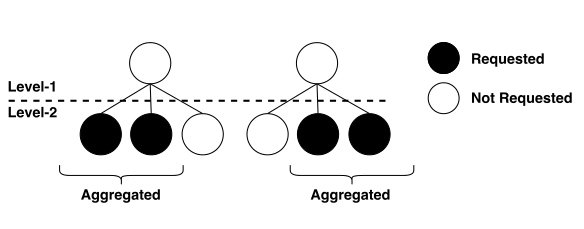
\includegraphics[scale=0.5]{Figs/tree.png}
\caption{A Practical Request Scenario in the Hierarchical Setting}
\label{fig:agg}
\end{figure*}




\subsection{Security of Hierarchical KAC}
\label{subsec:securityhierarchical}

For the CPA security of hierarchical KAC, we state the following theorem.
\begin{Theorem}
\label{th:hierarchicalCPA}
Let $\mathbb{G}_1$ and $\mathbb{G}_2$ be bilinear elliptic curve subgroups of prime order $q$. For any pair of positive integers $n',n (n'>n)$, the hierarchical KAC is $(\tau,\epsilon,n')$ CPA secure if the decision $(\tau,\epsilon,n,n)$-BDHE assumption holds in $(\mathbb{G}_1,\mathbb{G}_2)$.
\end{Theorem}

\noindent Once again, the proof of this theorem is very similar to the proof of Theorem \ref{th:basicCPA} and is hence avoided. Additionally, the hierarchical KAC scheme can also be easily modified to obtain a CCA-secure hierarchical KAC along similar lines to the discussion in Section \ref{sec:CCA}.

\subsection{Owner-Defined Hierarchy}
\label{subsec:owner}

The hierarchical KAC described above fixes the number of hierarchy levels to a pre-defined quantity $K$. This means any path in the hierarchy tree from the root to the length is of length $K+2$. However, in a realistic scenario, it is easy to see that a data owner may want to have her own hierarchical construction and customize the number of levels in the hierarchy. The existing construction of hierarchical KAC can be easily adopted for this scenario by taking either of the following steps:

\begin{itemize}
 \item The system may have a pre-defined upper bound $K$ on the number of hierarchy levels. A data owner willing to go beyond this level must register again with a different set of public, private and access keys to share the additional data classes. A data owner with fewer hierarchy levels than $K$ can have some \emph{dummy nodes} that merely act as placeholders in the overall hierarchy.
 
 \item The other option is to have variable size indexes for different nodes depending on the depth of the hierarchical structure to which it belongs. As and when the hierarchy levels change, the length of index for each node in the hierarchy also changes. This system would require updating the index for each and every data class node in the hierarchy every time a new level is introduced or an old level is deleted. But it does avoid the use of dummy rounds, and allows the data owner the flexibility to increase the number of levels in the hierarchy.
\end{itemize}



\subsection{Advantage over Hierarchical Cryptosystems}
\label{subsec:advantage}


We end this section by pointing out that a major advantage of our proposed hierarchical KAC is that it avoids a significant pitfall of several existing hierarchical encryption based schemes \cite{akl1983cryptographic,ateniese2012provably}. In standard tree based hierarchical systems, granting access to the key corresponding to any node implicitly grants access to all the keys in the subtree rooted at that node. This means granting access to a selected set of nodes in a given subtree would blow up the key-size to be the same as the number of nodes. This is avoided in our two-tier scheme, since decryption rights to any number of nodes (data classes) rooted at a particular node of the hierarchy tree may be aggregated into a single key corresponding to that node. Figure \ref{fig:agg} summarizes this phenomenon for a simple two-level hierarchical system. In the situation depicted, a tree-based hierarchy system would require $4$ constant size decryption keys, while our proposed hierarchical scheme would require only $2$ constant-size decryption keys. The savings is much more pronounced as the number of hierarchy levels increase, as depicted in the following section via simulation studies in practical deployment scenarios.


